\documentclass[tikz,border=4pt]{standalone}
\usepackage{tikz}
\usetikzlibrary{shapes.geometric,arrows.meta,positioning}
\begin{document}
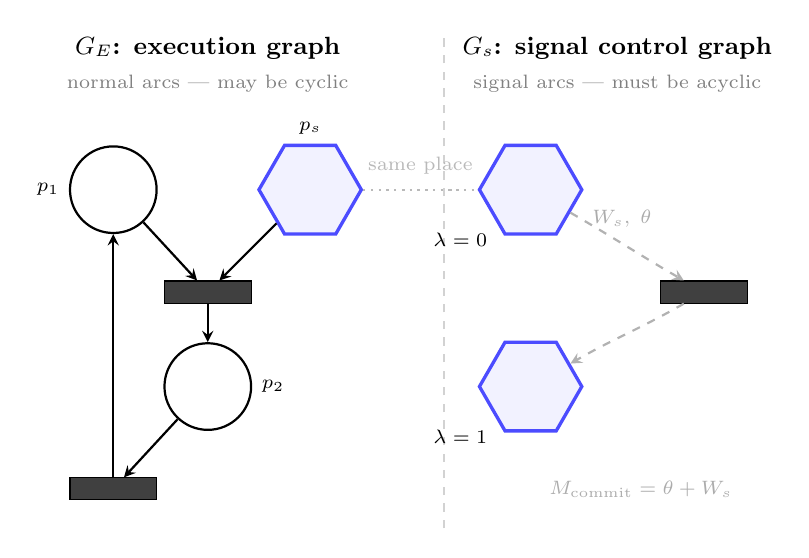
\begin{tikzpicture}[
  place/.style={circle, draw=black, thick, minimum size=1.1cm},
  sigplace/.style={regular polygon, regular polygon sides=6,
                   draw=blue!70, very thick, minimum size=1.3cm, fill=blue!5},
  bar/.style={rectangle, draw=black, fill=black!75,
              minimum width=1.1cm, minimum height=0.28cm},
  arr/.style={->, >=stealth, line width=0.8pt},
  sarr/.style={->, >=stealth, dashed, draw=gray!60, line width=0.8pt},
  every label/.style={font=\scriptsize}
]

%% ---- LEFT PANEL: G_E (execution graph) ----
\node[font=\small\bfseries] at (1.7, 6.1) {$G_E$: execution graph};
\node[font=\scriptsize, text=gray, align=center] at (1.7, 5.65)
     {normal arcs --- may be cyclic};

\node[place,    label={[font=\scriptsize]left:$p_1$}]   (p1) at (0.5, 4.3) {};
\node[sigplace, label={[font=\scriptsize]above:$p_s$}]  (ps) at (3.0, 4.3) {};
\node[bar]                                               (t1) at (1.7, 3.0) {};
\node[place,    label={[font=\scriptsize]right:$p_2$}]  (p2) at (1.7, 1.8) {};
\node[bar]                                               (t2) at (0.5, 0.5) {};

\draw[arr] (p1)       -- (t1);
\draw[arr] (ps)       -- (t1);
\draw[arr] (t1)       -- (p2);
\draw[arr] (p2) -- (t2);
\draw[arr] (t2) -- (p1);

%% ---- DIVIDER ----
\draw[dashed, gray!35, thick] (4.7, 0.0) -- (4.7, 6.3);

%% ---- RIGHT PANEL: G_s (signal control graph) ----
\node[font=\small\bfseries] at (6.9, 6.1) {$G_s$: signal control graph};
\node[font=\scriptsize, text=gray, align=center] at (6.9, 5.65)
     {signal arcs --- must be acyclic};

\node[sigplace, label={[font=\scriptsize]below left:$\lambda=0$}] (ps0) at (5.8, 4.3) {};
\node[sigplace, label={[font=\scriptsize]below left:$\lambda=1$}] (ps1) at (5.8, 1.8) {};
\node[bar]                                                         (tc)  at (8.0, 3.0) {};

\draw[sarr] (ps0) to[out=330, in=150]
     node[above=2pt, font=\scriptsize, text=gray!65, pos=0.45] {$W_s,\;\theta$}
     (tc);
\draw[sarr] (tc) to[out=210, in=30]
     (ps1);

\node[font=\scriptsize, text=gray!65, align=center] at (7.2, 0.5)
     {$M_{\mathrm{commit}} = \theta + W_s$};

%% ---- BRIDGE: same signal place in both panels ----
\draw[dotted, line width=0.8pt, gray!55] (ps.east) to[out=0, in=180]
     node[above=2pt, font=\scriptsize, pos=0.5] {same place}
     (ps0.west);

\end{tikzpicture}
\end{document}
